\documentclass[10pt]{beamer}
\usepackage{CJKutf8}
\usetheme[progressbar=frametitle]{metropolis}
\usepackage{appendixnumberbeamer}

\usepackage{booktabs}
\usepackage[scale=2]{ccicons}

\usepackage{pgfplots}
\usepgfplotslibrary{dateplot}
\usepackage{esvect}


\usepackage{graphicx}
\usepackage{subcaption}
\usepackage{tikz-qtree}
\usepackage{tikz-qtree-compat}
\usepackage{color}
\usepackage{upgreek}

\usepackage{xspace}
\newcommand{\themename}{\textbf{\textsc{metropolis}}\xspace}

\title{Info Graphical Models}
\subtitle{A General-purpose Graphical Model Framework}
\date{\today}
% \date{}
\author{Gong Heyang}
\institute{University of Science and Technology of China}
\titlegraphic{\hfill
\includegraphics[height=1.5cm]{logo.pdf}}

\begin{document}
\begin{CJK*}{UTF8}{gbsn}

\maketitle


\begin{frame}{修改意见}
    \begin{itemize}
        \item 文字太多,文字太多,多放图文字应该在脑子中。
        \item 少字,多图,重点要突出。我的 slide 本质是帮助自己书写论文。
    \end{itemize}
\end{frame}

\begin{frame}{Table of Contents}
  \setbeamertemplate{section in toc}[sections numbered]
  \tableofcontents%[hideallsubsections]
\end{frame}

\section[Intro]{Introduction}

\begin{frame}{Why Graphical Models}

    A “model,” in the common use of the word, is an idealized representation of reality that highlights some aspects and ignores others\cite{Pearl2009}. We need to model problems for two main reasons:
    
    
    \begin{itemize}
        \item  It allows us to translate an unstructured real world problem in to a structured mathematical representation
        \item It allows us to isolate the problem (model representation) with it’s solution (algorithm), meaning once we have a mathematical model for our problem we can apply any algorithm to solve it, 
    \end{itemize}
    
    Real world scenarios are complex and often involves large no of variables. So many times a graphical representation helps us to visualize better and then we use graph theory to reduce the number of relevant combinations of all the participating variables to represent the high dimensional probability distribution model more compactly.
    % 我需要借用一下模型是什么,图模型的作用等等某个slide的内容。
    
    % A Model is a declarative representation of a real world scenario or a problem that we want to analysis. When I say declarative it means it’s not derived but declared or defined either by a domain expert using its domain knowledge of the problem or by using statical learning algorithms from historic data set, and then represented using any mathematical tools like graph or even simply by an equation.
\end{frame}


\begin{frame}{Probabilistic Graphical Models (PGMs)}
    A graphical model or probabilistic graphical model (PGM) or structured probabilistic model is a probabilistic model for which a graph expresses the conditional dependence structure between random variables. They are widely used in bioinformatics, robotics, vision, natural language processing and machine learning.
     
    The framework of PGMs provides a mechanism for exploiting structure in complex distributions to describe them compactly, and in a way that allows them to be constructed and utilized effectively. The two most common types of graphical models are Bayesian networks (also called belief networks or causal networks) and Markov networks (also called Markov random fields (MRFs))
    
    %PGMs use a graph-based representation as the basis for compactly encoding a complex distribution over a high-dimensional space.
    
    % There is a dual mathematical perspective that one can use to interpret the structure of graphs: conditional independence and factorization. The framework of PGMs has achieved a remarkable success across a variety of domains, from near-optimal codes for communication to the state-of-the-art in combinatorial optimization;these models are widely used in bioinformatics, robotics, vision, natural language processing and machine learning.
\end{frame}

\begin{frame}{Types of PGMs}
    There are many types of PGMs, including
    \begin{itemize}
        \item Naive Bayes classifier where we use a tree with a single root.
        \item A factor graph is a bipartite graph representing the factorization of a function. 
        \item A clique tree or junction tree is a tree of cliques, used in the junction tree algorithm.
        \item A chain graph is a graph which may have both directed and undirected edges, but without any directed cycles.
        \item An ancestral graph is a further extension, having directed, bidirected and undirected edges.
        \item A restricted Boltzmann machine is a bipartite generative model specified over an undirected graph.
    \end{itemize}
    We also use dynamic graphical models, such as dynamic Bayesian networks(DBNs), recurrent neural networks(RNNs). 
\end{frame}

\begin{frame}{Implementation of PGMs}
    In the recent years, Probabilistic programming (PP) is a programming paradigm in which probabilistic models are specified and inference for these models is performed automatically. It represents an attempt to unify probabilistic modeling and traditional general purpose programming in order to make the former easier and more widely applicable. Many probabilistic programming languages have been developed for PP, such as Pyro, Gen, Edward, which are based on a key mathematical concepts --- stochastic computation graphs (SCGs). SCGs are directed acyclic graphs that include both deterministic functions and conditional probability distributions which could assist researchers in developing intricate models involving a combination of stochastic and deterministic operations, enabling, for example, attention, memory, and control actions.  
\end{frame}


\begin{frame}{The Weakness of PGMs Framework}
    
    % learning and inference
    % 图结构难以找到,structure learning 非常困难。
    % 文献中总结一些弱点,其中一个突出的弱点是难以处理带环的图模型(例如markov 性质,因果理论)。强调出现这种情况的原因是表示能力不够,我们发展出来一个表示能力更加强大的框架。
    The framework of PGMs has achieved a remarkable success across a variety of domains, but it becomes very struggling while modeling complex problems with PGMs in many aspects, including
    
    \begin{itemize}
        \item representing many real-world complex systems compactly with existing graphical structures, 
        \item selecting a proper graphical structure for a given problem, and
        \item dealing with systems with feedback loops\cite{bongers2016theoretical}.
    \end{itemize}
    
    A kind of generalization of PGMs,  info graphical models (IGMs), is proposed which highlights the quantum and information view of complex systems. \textbf{And the new framework will help in alleviating the above difficulties, especially for dealing with systems with feedbacks.}   
    % thus interpretations of nodes and edges in the graph have been totally changed.  
    
\end{frame}

\section[IGMs]{The Framework of IGMs}

\subsection{Definitions}

\begin{frame}{What is IGMs?}
    \begin{quote}
    \emph{Info graphical models (IGMs)} is general-purpose framework for constructing probabilistic models of complex problems which can be deemed as a generalization of probabilistic graphical models (PGMs) in the interpretations of edges and nodes with a quantum and information view.        
    \end{quote}
 
    
    If the underlying graph structure is a directed graph, then we can define info directed graph models (IDGMs), formal definitions of IDGMs and IDMs are presented below. 
    
\end{frame}

\begin{frame}{Definition of IDGMs}
\begin{definition}[Info Graph Directed Models(IDGMs)]
    An \emph{info directed graph model(IDGM)} by definition consists of:
    \begin{enumerate}[a)]
        \item  A directed graph $G = (V, E)$ associated with a set of variables $X_V$. 
        \item  For every edge $e=(i, j) \in E$, there is a set of samples $S_e$(or $S_{ij}$) which represents the measured or observed information of $X_i$ that is called the state of edge $e$. Consequently, we denote $S_T = \{S_e\}_{e \in T}$ for $T\subseteq E$,  ). 
        \item  For every node $v \in V$, there is an information processing mechanism $f_v$ which collects information from its input edges $v^{in} = \{(k, v) \in E \}$ and forces $X_v \sim f_v(S_{v^{in}})$, then sends out by default measured or observed information $x_v$ to its output edges. 
    \end{enumerate}  
\end{definition}


For an acyclic IDGM $G$, if we let information $S_{ij}$ on every edge $(i, j) \in E$ depends only on current measurement or observation $\{X_i = x_i\}$, then $G$ is just a Bayesian network, and $f_v(S_{v^{in}})$ is simplified to the conditional density of $X_v$ given input variables $X_{v^{in}}$.

\end{frame}

\begin{frame}{Example of IDGMs}
    \metroset{block=fill}
    \begin{exampleblock}{Dynamic Baysian Network}
        An IDGM $G$ with nodes $X, Y, Z$ and egdes $(Z, Z), (Z, X), (Z, Y), (X, X), (X, Y)$ with corresponding edge information $z^{(t-1)}, z^{(t)}, z^{(t)}, x^{(t-1)}, x^{(t)}$. $G$ can be viewed as a dynamic Bayesian network.
    \end{exampleblock}
    \begin{columns}[T,onlytextwidth]
    \column{0.5\textwidth}
        \begin{figure}
            \centering
            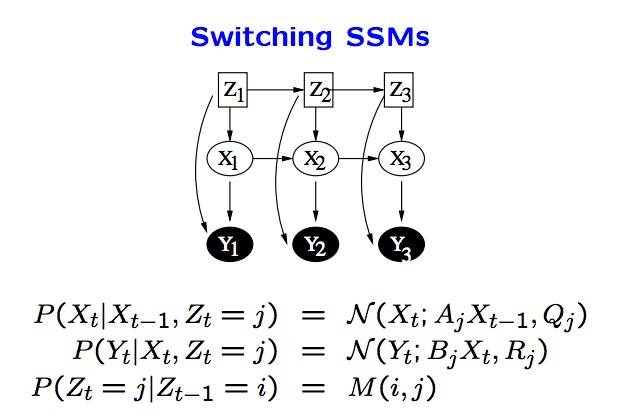
\includegraphics[width=4cm]{latex/image/dbn.jpg}
            \caption{IDGM}
            \label{fig:my_label}
        \end{figure}
    \column{0.5\textwidth}
        \begin{figure}
            \centering
            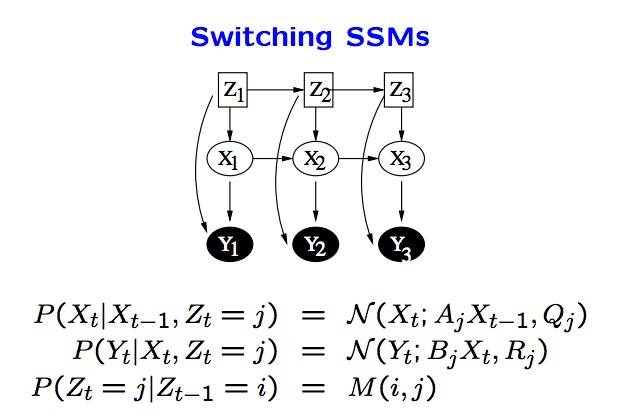
\includegraphics[width=4cm]{latex/image/dbn.jpg}
            \caption{Dynamic Bayesian network}
            \label{fig:dbn}
        \end{figure}
    \end{columns}
    
\end{frame}


\begin{frame}{Defintion of IGMs}
    The graphs in our framework are not restricted to the case of directed graphs\footnote{Actually, we don't restrict the type of underlying graph of an IGM which can be directed graph, undirected graph or even hyphgraph with corresponding interpretation.}. Consequently for any graph structure with certain definitions of input edges and output edges, we have:

\begin{definition}[Info Graph Models(IGMs)]
    An \emph{info graph model(IGM)} by definition consists of:
    \begin{enumerate}[a)]
        \item  A graph $G = (V, E)$ associated with a set of variables $X_V$. 
        \item  For every edge $e \in E$, there is a set $S_e$ which represents the  information from input nodes that is called the state of edge $e$. 
        \item  For every node $v \in V$, there is an information processing mechanism $f_v$ which accepts information $S_{v^{in}}$ from its input edges ${v^{in}}$ , then forcing $X_v \sim f_v(S_{v^{in}})$, and sends out information to its output edges. 
    \end{enumerate}  
\end{definition}
\end{frame}

\begin{frame}{Example of IDMs}
    \metroset{block=fill}
    \begin{exampleblock}{Ancestral Graphs}
        \begin{itemize}
            \item  Ancestral graphs are mixed graphs used with three kinds of edges: directed edges, drawn as an arrow from one vertex to another, bidirected edges, which have an arrowhead at both ends, and undirected edges, which have no arrowheads.
            \item Ancestral graphs models are a class of graphical models that are closed with respect to conditional independence under both marginalization and conditioning. 
            \item Ancestral graphs are causally interpretable but are restricted to conditional independence models. 
        \end{itemize}
        IDMs include ancestral graphs as special case.
    \end{exampleblock}
    
   % 画出图形就是关键,语言不必说明。
\end{frame}

\subsection{Interpretations}

\begin{frame}{Information Theory}

Typical examples of the communication system are line telegraphy, mobile communication etc..
    \begin{figure}
        \centering
        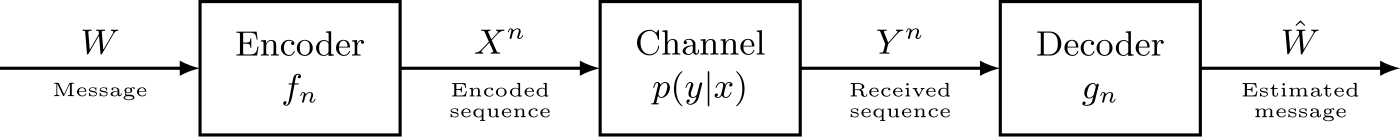
\includegraphics[width=0.8\textwidth]{latex/image/channel.png}
        \caption{The basic mathematical model for a communication system.}
        \label{fig:channel}
    \end{figure}
    
\begin{itemize}
    \item $W$ is the message to be transmitted, ${\hat  {W}}$ is the estimate of the transmitted message;
    \item $X/Y$ is the channel input/output symbol ($X^{n}/Y^{n}$ is a sequence of $n$ symbols) taken in an alphabet ${\mathcal {X}}/{\mathcal {Y}}$;
    \item ${\displaystyle p(y|x)=p_{Y|X}(y|x)}$ is the noisy channel, which is modeled by a conditional probability distribution; and,
    \item  $f_{n}/g_{n}$ is the encoding/decoding function for a block of length $n$.
\end{itemize}







    
\end{frame}

\begin{frame}{Symmetrical View of Nodes and Edges}
    
    In the framework of IGMs: 
    \metroset{block=fill}
    \begin{block}{Principle 1}
    \label{prin:sym}
     Nodes are affected by information from its input edges, and edges collect information from its input nodes.
    \end{block}
    
    Actually, this symmetrical treatment is originated from a formal mathematical concept --- hypergraph. Contrast to commonly used graphs which define edges between two different nodes, a graph that allows edges connect a set of nodes(called hyperedges, e.g. self-loops) is referred as \emph{hypergraph} with the mathematical symmetrical property of edges and nodes, which have been extensively used in machine learning tasks as the data model and classifier regularization\cite{zhou2007learning}.    
\end{frame}


\begin{frame}{It from Qubit}
    
    In the framework of IGMs: 
    \metroset{block=fill}
    \begin{block}{Principle 2}
    \label{prin:quantum}
    Every node represents a quantum state that evolves according to its environment information.
    \end{block}
    All Information are on edges and nodes state associate with a "collapse" distribution according to this principle.

    
\end{frame}

\section{Representation}


% \subsection{Markov Property}

\begin{frame}{Graphical Representation}
    An idea graphical models framework should allow us to choreograph a parsimonious and modular representation of the domain knowledge of variety complex problems, interrogate that representation and finally answer inferential questions correctly with ease. \textbf{\emph{The Markov property plays a central role in PGMs for efficient computation}}
    % 表示能力
  
\end{frame}


\begin{frame}{Independent Mechanisms}
    \metroset{block=fill}
    \begin{block}{Principle 3}
    \label{prin:indep}
    For any two disjoint sets of variables $X, Y$ in  an IGM, $X$ and $Y$ are conditionally independent given their information from the corresponding input edges.
    \end{block}
    
    The modeling principle for IGMs is corresponding to the Markov property of PGMs.
    
\end{frame}

\usetikzlibrary{arrows}
\usetikzlibrary{arrows.meta, calc}
\usetikzlibrary{shapes,positioning,decorations.markings}
\usetikzlibrary{arrows, automata, chains, positioning, shapes.geometric, shapes.symbols}
\usetikzlibrary{shapes,decorations,arrows,calc,arrows.meta,fit,positioning}
\tikzset{
	-Latex, auto, node distance =1 cm and 1 cm, semithick,
	state/.style ={ellipse, draw, minimum width = 0.7 cm},
	point/.style = {circle, draw, inner sep=0.04cm, fill, node contents={}},
	bidirected/.style={Latex-Latex, dashed},
	el/.style = {inner sep=2pt, align=left, sloped}
}

\begin{frame}{Cyclic Directed Graphs}
    In the framework of IGMs, directed graphs with cycles would have a natural interpretation. 
    
    \metroset{block=fill}
    \begin{exampleblock}{Example}
    \label{exmp:feelback}
    An info graphical model $G=(V, E)$ with nodes $A, B, C \in V$ and three directed edges $\vv{AB}, \vv{BC}, \vv{CA} \in E$ which forms a cycle.
    \end{exampleblock}
        \begin{figure}[h]
	\begin{subfigure}[tb]{0.45\textwidth}
		\centering
		\begin{tikzpicture}
		\node[state] (x) at (0, 0) {$X_A$};
		\node[state] (z) at (2, 2) {$X_C$};
		\node[state] (y) at (4, 0) {$X_B$};
		
		% Directed edge
		\path (x) edge[bend right=10, align=right, above] node {$x_A^{(t)}$} (y);
		\path (y) edge[bend right=10, align=left, above] node {$x_C^{(t)}$} (z);
		\path (z) edge[bend right=10, align=left, above] node {$x_B^{(t)}$} (x);
		\end{tikzpicture}
		\caption{Case 1: Information on edges are just a sample of its input nodes.}
		\label{fig:onesample}
	\end{subfigure}
    \hfill
	\begin{subfigure}[tb]{0.45\textwidth}
		\centering
		\begin{tikzpicture}
		\node[state] (x) at (0, 0) {$X_A$};
		\node[state] (z) at (2, 2) {$X_C$};
		\node[state] (y) at (4,0) {$X_B$};
		
		% Directed edge
		\path (x) edge[bend right=10, align=right, above] node {$\{x_A^{(t)}, x_A^{(t-1)}, ...\}$} (y);
		\path (y) edge[bend right=10, align=left, above] node {$\{x_B^{(t)}, x_B^{(t-1)}, ...\}$} (z);
		\path (z) edge[bend right=10, align=left, above] node {$\{x_C^{(t)}, x_C^{(t-1)}, ...\}$} (x);
		\end{tikzpicture}
		\caption{Case 2: Information on edges are a sequence of samples of its input nodes.}
		\label{fig:manysamples}
	\end{subfigure}\caption{Cyclic IGM Example.}
\end{figure}
\end{frame}



\begin{frame}{Update Rules}
    Let $S_{v}^{(t)}$ denote the information from input edges of node $v$ and $x_v^{(t)}$ is a sample of $X_v^{(t)}$. For Case 1 in Fig \ref{fig:onesample}, 
    \begin{columns}[T,onlytextwidth]
    \column{0.45\textwidth}
    \alert{How nodes evolve according to information from input edges?}
    \begin{equation*} \label{eq:evolve}
    \left\{
         \begin{array}{lr}
         X_A^{(t+1)} \sim f_A(x_A|S_{A}^{(t)}) &  \\
         X_B^{(t+1)} \sim f_B(x_B|S_{B}^{(t)}) & \\
         X_C^{(t+1)} \sim f_C(x_C|S_{C}^{(t)}) &  
         \end{array}
    \right.
    \end{equation*}
    
    \column{0.45\textwidth}
    \alert{How edges collect information from their input nodes?}
    \begin{equation*} \label{eq:collect}
    \left\{
         \begin{array}{lr}
         S^{(t+1)}_A = \{x_C^{(t+1)}\} \\
         S^{(t+1)}_B = \{x_A^{(t+1)}\}\\
         S^{(t+1)}_C = \{x_B^{(t+1)}\}  
         \end{array}
    \right.
    \end{equation*}


  \end{columns}
  
    For the more complex case in Fig \ref{fig:manysamples}, 
    \begin{columns}[T,onlytextwidth]
    \column{0.45\textwidth}
    \begin{equation*} \label{eq:evolve}
    \left\{
         \begin{array}{lr}
         X_A^{(t+1)} \sim f_A(x_A|S_{A}^{(t)}) &  \\
         X_B^{(t+1)} \sim f_B(x_B|S_{B}^{(t)}) & \\
         X_C^{(t+1)} \sim f_C(x_C|S_{C}^{(t)}) &  
         \end{array}
    \right.
    \end{equation*}
    
    \column{0.45\textwidth}
    \begin{equation*} \label{eq:collect}
    \left\{
     \begin{array}{lr}
     S^{(t+1)}_A = S_{A}^{(t)} \cup \{x_C^{(t+1)}\} \\
     S^{(t+1)}_B = S_{B}^{(t)} \cup \{x_A^{(t+1)}\}\\
     S^{(t+1)}_C = S_{C}^{(t)} \cup \{x_B^{(t+1)}\}  
     \end{array}
    \right.
    \end{equation*}
  \end{columns}
\end{frame}


\begin{frame}{Update rules for IGMs}

Let $G=(V, E)$ be an IGM, then for every nodes $v\in V$, we have 
$$
X_v^{(t+1)} \sim f_v(S_{v^{in}}^{(t)}),
$$

and for every edge $e \in E$

$$
S_e^{(t+1)} = S_e^{(t)} \cup \mathrm{info}(X_{e^{in}}^{(t+1)})
$$

where $v^{in}$ stands for input edges of node $v$ and $e^{in}$ stands for input nodes of edge $e$. And $\mathrm{info}(X_{e^{in}}^{(t+1)})$ is the information collected or measured by edge $e$, which can be a sample or some other measured information from nodes $e^{in}$.

\end{frame}


\begin{frame}{PID Control Systems}
\begin{figure}[h]
	\begin{subfigure}[tb]{0.45\textwidth}
		\centering
        \begin{tikzpicture}[auto, node distance=1.2cm,>=latex']
            \tikzstyle{block} = [draw, fill=white, rectangle, 
                minimum height=3em, minimum width=4em]
            \tikzstyle{sum} = [draw, fill=white, circle, node distance=1cm]
            \tikzstyle{input} = [coordinate]
            \tikzstyle{output} = [coordinate]
            \tikzstyle{pinstyle} = [pin edge={to-,thin,black}]
            \node [input, name=input] {};
            \node [sum, right of=input] (sum) {};
            \node [block, right of=sum] (controller) {$Control$};
            \node [block, right of=controller,
            pin={[pinstyle]above:Disturbances},
                    node distance=2cm] (system) {$Process$};
        
            \draw [->] (controller) -- node[name=u] {$u^{(t)}$} (system);
            \node [output, right of=system] (output) {};
            \node [input, below of=u] (measurements) {Measurements};
        
            \draw [draw,->] (input) -- node {$r^{(t)}$} (sum);
            \draw [->] (sum) -- node {} (controller);
            \draw [->] (system) -- node [name=y] {}(output);
            \draw [->] (y) |- (measurements);
            \draw [->] (measurements) -| node[pos=0.99] {$-$} 
                node [near end] {$y^{(t)}$} (sum);
 
        \end{tikzpicture}
		\caption{A typical PID control system.}
		\label{fig:pid1}
	\end{subfigure}
    \hfill
	\begin{subfigure}[tb]{0.5\textwidth}
		\centering
    	\begin{tikzpicture}
    	\node[state, shape=rectangle] (x) at (0, 0) {$U$};
    	\node[state] (y) at (4, 0) {$Y$};
    	\path (x) edge[bend right=0, align=right, above] node {$u^{(t)}$} (y);
    	\path (y) edge[bend right=60, align=left, above] node {$\{y^{(t)}, y^{(t-1)}, ... \}$} (x);
    	\end{tikzpicture}
		\caption{IGM view of typical PID control system}
		\label{fig:pid2}
	\end{subfigure}\caption{PID Control System as an IGM.}
\end{figure}

A PID controller is an instrument used in industrial control applications to regulate temperature, flow, pressure, speed and other process variables. PID (proportional integral derivative) controllers use a control loop feedback mechanism to control process variables and are the most accurate and stable controller. 

\end{frame}


\begin{frame}{Update rules for PID}

\begin{equation}
\label{eq:pid}
    u^{(t)}=K_{\text{p}} e^{(t)}+K_{\text{i}}\sum_{t'\leq t}e^{(t')}\, +K_{\text{d}} \Delta e^{(t)},  
\end{equation}


where $K_{\text{p}}, K_{\text{i}}$, and $K_{\text{d}}$, all non-negative, denote the coefficients for the proportional, integral, and derivative terms respectively (sometimes denoted $P$, $I$, and $D$).

If we treat PID as an IGM, the updating rules are

    \begin{columns}[T,onlytextwidth]
    \column{0.45\textwidth}
    \begin{equation*} 
    \left\{
         \begin{array}{lr}
         Y^{(t+1)} \sim f_Y(y|S_{Y^{in}}^{(t)}) &  \\
         U^{(t+1)} \sim f_U(u|S_{U^{in}}^{(t)}) & 
         \end{array}
    \right.
    \end{equation*}
    
    \column{0.45\textwidth}
    \begin{equation*} \label{eq:collect}
    \left\{
     \begin{array}{lr}
     S^{(t+1)}_{Y^{in}} = \{u^{(t+1)}\} \\
     S^{(t+1)}_{U^{in}} = S_{U^{in}}^{(t)} \cup \{y^{(t+1)}\}\\
     \end{array}
    \right.
    \end{equation*}
  \end{columns}
  where $f_Y$ is determined by the system itself and $f_U$ is a Dirac density at point determined by Formula \ref{eq:pid}.
  
  


\end{frame}

\section{IGMs for Complex Systems}

\begin{frame}{Complex Systems}
    Complex systems are characterized by the presence of multiple interrelated aspects, many of which relate to the reasoning task. IGMs have shown their advantage on overcome theoretical impediments on systems with cycles, and we now also show example how it facilitate modeling of complex empirical science problems.
\end{frame}

\begin{frame}{Agent-based Models}

An agent-based model (ABM) is a class of computational models for simulating the actions and interactions of autonomous agents with a view to assessing their effects on the system as a whole, which is widely used in many empirical science such as social science and economics. 

\end{frame}

\begin{frame}{ABM in Eoconomic}

Leigh Tesfatsion summarize five essential properties in real-world economies, 

\begin{itemize}
    \item  First, they consist of heterogeneous interacting participants characterized by distinct local states (data, attributes, methods) at each given time. 
    \item Second, they are open-ended dynamic systems whose dynamics are driven by the successive interactions of their participants. 
    \item Third, human participants are strategic decision-makers whose decision processes take into account past actions and potential future actions of other participants. 
    \item Fourth, all participants are locally constructive, i.e., constrained to act on the basis of their own local states at each given time. 
    \item Fifth, the actions taken by participants at any given time affect future local states and hence induce system reflexivity.
\end{itemize}
    
\end{frame}

\begin{frame}{Five Properties}
    The five properties can be naturally interpreted in IGMs framework:
    
    \begin{itemize}
    \item First, heterogeneous nodes interacting by sending and accepting information on edges.
    \item Second, nodes evolve according to edges information and edges collect information from nodes intrinsically imply a dynamic process. % according to updating rules.
    \item Third, nodes evolve according to mechanism functions $f_v$ which take collected the input edges information (which could include both present and past information) as inputs.
    \item Fourth, nodes are independently affected by information from its inputs information locally.
    \item Reflexivity refers to circular or feedback loops which has been discussed in previous Section \ref{sec:repre}.
\end{itemize} 

\end{frame}

\section{Conclusion}

\begin{frame}{Summary}

%   Get the source of this theme and the demo presentation from

%   \begin{center}\url{github.com/matze/mtheme}\end{center}

%   The theme \emph{itself} is licensed under a
%   \href{http://creativecommons.org/licenses/by-sa/4.0/}{Creative Commons
%   Attribution-ShareAlike 4.0 International License}.

%   \begin{center}\ccbysa\end{center}

\end{frame}

{\setbeamercolor{palette primary}{fg=black, bg=yellow}
\begin{frame}[standout]
  Questions?
\end{frame}
}

\appendix

\begin{frame}[fragile]{Backup slides}
%   Sometimes, it is useful to add slides at the end of your presentation to
%   refer to during audience questions.

%   The best way to do this is to include the \verb|appendixnumberbeamer|
%   package in your preamble and call \verb|\appendix| before your backup slides.

%   \themename will automatically turn off slide numbering and progress bars for
%   slides in the appendix.
\end{frame}

\begin{frame}[allowframebreaks]{References}

\bibliography{egbib}
\bibliographystyle{abbrv}

\end{frame}


\end{CJK*}
\end{document}
